\providecommand{\econtexRoot}{}
\renewcommand{\econtexRoot}{..}
\providecommand{\econtexPaths}{}\renewcommand{\econtexPaths}{\econtexRoot/Resources/econtexPaths}
% The \commands below are required to allow sharing of the same base code via Github between TeXLive on a local machine and Overleaf (which is a proxy for "a standard distribution of LaTeX").  This is an ugly solution to the requirement that custom LaTeX packages be accessible, and that Overleaf seems to ignore symbolic links (even if they are relative links to valid locations)
\providecommand{\econtex}{\econtexRoot/Resources/texmf-local/tex/latex/econtex}
\providecommand{\econtexSetup}{\econtexRoot/Resources/texmf-local/tex/latex/econtexSetup}
\providecommand{\econtexShortcuts}{\econtexRoot/Resources/texmf-local/tex/latex/econtexShortcuts}
\providecommand{\econtexBibMake}{\econtexRoot/Resources/texmf-local/tex/latex/econtexBibMake}
\providecommand{\econtexBibStyle}{\econtexRoot/Resources/texmf-local/bibtex/bst/econtex}
\providecommand{\econtexBib}{economics}
\providecommand{\notes}{\econtexRoot/Resources/texmf-local/tex/latex/handout}
\providecommand{\handoutSetup}{\econtexRoot/Resources/texmf-local/tex/latex/handoutSetup}
\providecommand{\handoutShortcuts}{\econtexRoot/Resources/texmf-local/tex/latex/handoutShortcuts}
\providecommand{\handoutBibMake}{\econtexRoot/Resources/texmf-local/tex/latex/handoutBibMake}
\providecommand{\handoutBibStyle}{\econtexRoot/Resources/texmf-local/bibtex/bst/handout}

\providecommand{\FigDir}{\econtexRoot/Figures}
\providecommand{\CodeDir}{\econtexRoot/Code}
\providecommand{\DataDir}{\econtexRoot/Data}
\providecommand{\SlideDir}{\econtexRoot/Slides}
\providecommand{\TableDir}{\econtexRoot/Tables}
\providecommand{\ApndxDir}{\econtexRoot/Appendices}

\providecommand{\ResourcesDir}{\econtexRoot/Resources}
\providecommand{\rootFromOut}{..} % Path back to root directory from output-directory
\providecommand{\LaTeXGenerated}{\econtexRoot/LaTeX} % Put generated files in subdirectory
%\providecommand{\EqDir}{\econtexRoot/Equations} % Put generated files in subdirectory
\providecommand{\EqDir}{Equations} % Put generated files in subdirectory
\providecommand{\econtexPaths}{\econtexRoot/Resources/econtexPaths}
\providecommand{\LaTeXInputs}{\econtexRoot/Resources/LaTeXInputs}
\providecommand{\LtxDir}{LaTeX/}

\documentclass[pdflatex]{beamer}\providecommand{\texname}{BufferStockTheory-Slides}% Indicate the keyname for the bibtex entry corresponding to this document
\newif\ifdvi\dvifalse

%\usepackage{optional}
\usepackage{ifthen}%\usepackage{\econtexRoot/BufferStockTeory}

% Can't read in BufferStockTheory.sty because some packages conflict with Beamer
% So need to redefine everything here

\usepackage{\econtexShortcuts}
\usepackage{natbib,amsmath,amssymb,rotating,subfigure}
\usepackage{verbatim,moreverb,graphicx}
\usepackage{wasysym}
\usepackage{dcolumn}
\usepackage{cancel}
%\providecommand{\LtxDir\EqDir}{\econtexRoot/Equations}
\providecommand{\FigsRaw}{\econtexRoot/Code/Python/Figures}
\providecommand{\CodeDir}{\econtexRoot/Code}
\providecommand{\CalibrationDir}{\econtexRoot/Calibration}
\providecommand{\TableDir}{\econtexRoot/Tables}
\providecommand{\ApndxDir}{\econtexRoot/Appendices}
\providecommand{\Ex}{\mathbb{E}}

%\usepackage{natbib}\newcommand*{\newblock}{}

\mode<presentation>
{
  \usetheme{Warsaw}
  % or ...
  \setbeamercovered{transparent}
}

%\beamerdefaultoverlayspecification{<+->}

%\setbeamertemplate{navigation symbols}{}  % Take away navigation symbols

\usetheme{Warsaw}

\setbeamersize{text margin left=3mm}
\setbeamersize{text margin right=3mm}


%_____________ Opening slide _______________________

\title[Buffer Stock Theory]{Theoretical Foundations of Buffer Stock Saving}
\author[Carroll]{Chris Carroll}
\institute[JHU]{Johns Hopkins University}
\date[\today]{September 12, 2019  \\ \medskip \medskip \medskip \href{https://econ-ark.org/}{\small Powered By} \\ 
\includegraphics[width=0.5in]{\econtexRoot/Resources/econ-ark-logo-small.png}}

\begin{document}\bibliographystyle{\econtexBibStyle}

\begin{frame}[plain]
  \titlepage
\end{frame}


%_____________ 1st section  ____________
\section{Introduction}
\subsection{Motivation}

\begin{frame}
\frametitle{Drawbacks of Numerical Solutions}


\pause A Black Box \pause
\begin{itemize}
\item Can Construct Solution to Model Without Really Understanding It
\item Hard Even To Be Sure Your Numerical Solution Is {\it Right}
\item Little Intuition for How Results Might Change With
\begin{itemize}
\item Calibration
\item Structure
\end{itemize}
\item {\it Very} Hard To Teach!
\end{itemize}

\medskip\medskip
\pause I Am A {\it Big} Fan Of Numerical Methods
\begin{itemize}
\item Have Done A Good Deal Of Work With Them Myself
\item But As A Result, Have Felt All These Drawbacks Keenly
\end{itemize}



\end{frame}

\begin{frame}
\frametitle{The Gap This Paper Fills}

\pause Foundations For Microeconomic Household's Problem With
\begin{itemize}
\item Uncertain Labor Income
\item No Liquidity Constraints
\item CRRA Utility
\item (Problem with Liquidity Constraints Is A Limiting Case)
\end{itemize}

\end{frame}
\begin{frame}{Key Result}
\pause
Restrictions On Parameter Values Such That \pause
\begin{itemize}
\item Problem Defines A Contraction Mapping
\begin{itemize}
\item $\Rightarrow~~\exists $ A Unique Consumption Function $\cFunc(m)$
\end{itemize}
\item There Is A `Target' Ratio Of Assets to Permanent Income
\begin{itemize}
\item Requires A Key `Impatience' Condition To Hold
\item Good News
\begin{itemize} \item Condition Is Weaker (Easier To Satisfy) Than Previous Papers Imposed \end{itemize}
\end{itemize}
\end{itemize}

\end{frame}

\section{The Problem}

\begin{frame}

Limit as horizon $T$ goes to infinity of 
%\input \LtxDir\EqDir/supfn

\input \LtxDir\EqDir/DBCparts

\input \LtxDir\EqDir/tShkDef

\begin{itemize}
\item $\util(\bullet)=\bullet^{1-\CRRA}/(1-\CRRA)$; $\Ex_{t}[\pShk_{t+n}]=\Ex_{t}[\tShk_{t+n}]=1~\forall~n>0$; $\beta < 1, \CRRA > 1$
\end{itemize}

\end{frame}

\begin{frame}
\frametitle{Surely This Problem Has Been Solved?}

\pause No.
\begin{itemize}
\item Can't Use Stokey et.\ al.\ theorems because CRRA utility
\item Lit thru \cite{mnUnique} Can't Handle Permanent Shocks
\item Must Use Boyd's `Weighted' Contraction Mapping Theorem 
\item Surprisingly Subtle
\end{itemize}

\pause Fortunately, the Conclusions Are Simple!

\end{frame}

\subsection{The Perfect Foresight Problem}

\begin{frame}
\frametitle{Benchmark: Perfect Foresight Model}

Definitions: \smallskip

\begin{tabular}{llcl}
   Absolute Patience Factor & $\Pat$ & = & $(\Rfree \Discount)^{1/\CRRA}$
\\ Return Patience Factor & $\PatR$ & = & \Pat/\Rfree
\\ Perfect Foresight Growth Patience Factor & $\PatPGro$ & = & \Pat/\PGro
\end{tabular}

\medskip

\begin{tabular}{l|lcl|l} \hline
   Name                                 & \multicolumn{3}{c|}{Condition}    & Implication 
\\ \hline (\AIC) Absolute Impatience Condition  & $\Pat$  & $<$ & 1 & $\cLev$ $\downarrow$ over time
\\ (\RIC) Return Impatience Condition    & $\PatR$ & $<$ & 1 & $\cLev/\aLev$ $\downarrow$ over time
\\ (\GIC) Growth Impatience Condition & $\PatPGro$ & $<$ & 1 & $\cLev/\pLev$ $\downarrow$ over time
\end{tabular}

\medskip

\end{frame}

\begin{frame}
\frametitle{When Does A Useful Limiting Solution Exist?}

Finite Human Wealth (\FHWC) condition:
\begin{eqnarray}
\PGro & < & \Rfree
\end{eqnarray}

\pause\medskip
Return Impatience Condition:
\begin{eqnarray}
\PatR & < & \Rfree
\end{eqnarray}

\end{frame}

\begin{frame}
\frametitle{What If There Are Liquidity Constraints?}

\pause 

\begin{itemize}
\item \FHWC~is {\it not} necessary for solution to exist
\item Other Key Condition For Useful Solution is

`Perfect Foresight Finite Value of Autarky Condition (\PFFVAC)':
\begin{eqnarray}
\beta \PGro^{1-\CRRA} & < & 1  
\end{eqnarray}

\item Without \RIC, Constraints Are Irrelevant
\begin{itemize}
\item Because Wealth Always Wants To Rise, So Constraint Never Binds
\end{itemize}
\end{itemize}

\end{frame}

\begin{frame}
\frametitle{Liquidity Constraints and Uncertainty}

\begin{itemize}
\item Introduce permanent shocks to income
\item Finite Value of Autarky Condition Becomes
\input \LtxDir\EqDir/FVAC
\end{itemize}

\end{frame}



\subsection{The Real Problem}
\begin{frame}
\frametitle{Contraction Mapping Requirements}

Finite Value of Autarky Condition: Same As In Liq Constr Problem!
\input \LtxDir\EqDir/FVAC

`Weak Return Impatience Condition' (\WRIC)

\begin{eqnarray}
 0 \leq & \pZero^{1/\CRRA} \PatR & < 1 \label{eq:WRIC}
\end{eqnarray}

\end{frame}

\begin{frame}
\frametitle{Requirement For Existence Of A Target}

Definitions: `Uncertainty-Adjusted' Growth:
\input \LtxDir\EqDir/PGroAdj

Adjusted Growth Patience Factor:
\input \LtxDir\EqDir/PatPGroAdj

Growth Impatience Condition:
\input \LtxDir\EqDir/GICNrm~



Why?  Because it can be shown that
\begin{eqnarray}
 \lim_{m_{t} \rightarrow \infty} \Ex_{t}\left[\frac{\mRat_{t+1}}{\mRat_{t}}\right] & = & \PatPGroAdj  \label{eq:mGrowth}
\end{eqnarray}

\end{frame}

\section{Features Of the Solution}
\subsection{Five Propositions}
\begin{frame}
\frametitle{Five Propositions}

\begin{enumerate}
\item $\lim_{m_{t} \rightarrow \infty} \Ex_{t}[\cLev_{t+1}/\cLev_{t}] = \Pat$
\item $\lim_{m_{t} \rightarrow 0} \Ex_{t}[\cLev_{t+1}/\cLev_{t}] = \infty$
\item $\exists$ a unique target value of $m$, called $\check{m}$
\item $\Ex_{t}[\cLev_{t+1}/\cLev_{t} | m_{t} = \check{m}] = \PGro - \epsilon$
\item $\left(\frac{d \Ex_{t}[\cLev_{t+1}/\cLev_{t}]}{d m_{t}}\right) < 0$
\end{enumerate}

\end{frame}

\subsection{The Target Saving Figure}
\begin{frame}
\frametitle{The Target Saving Figure}
\centerline{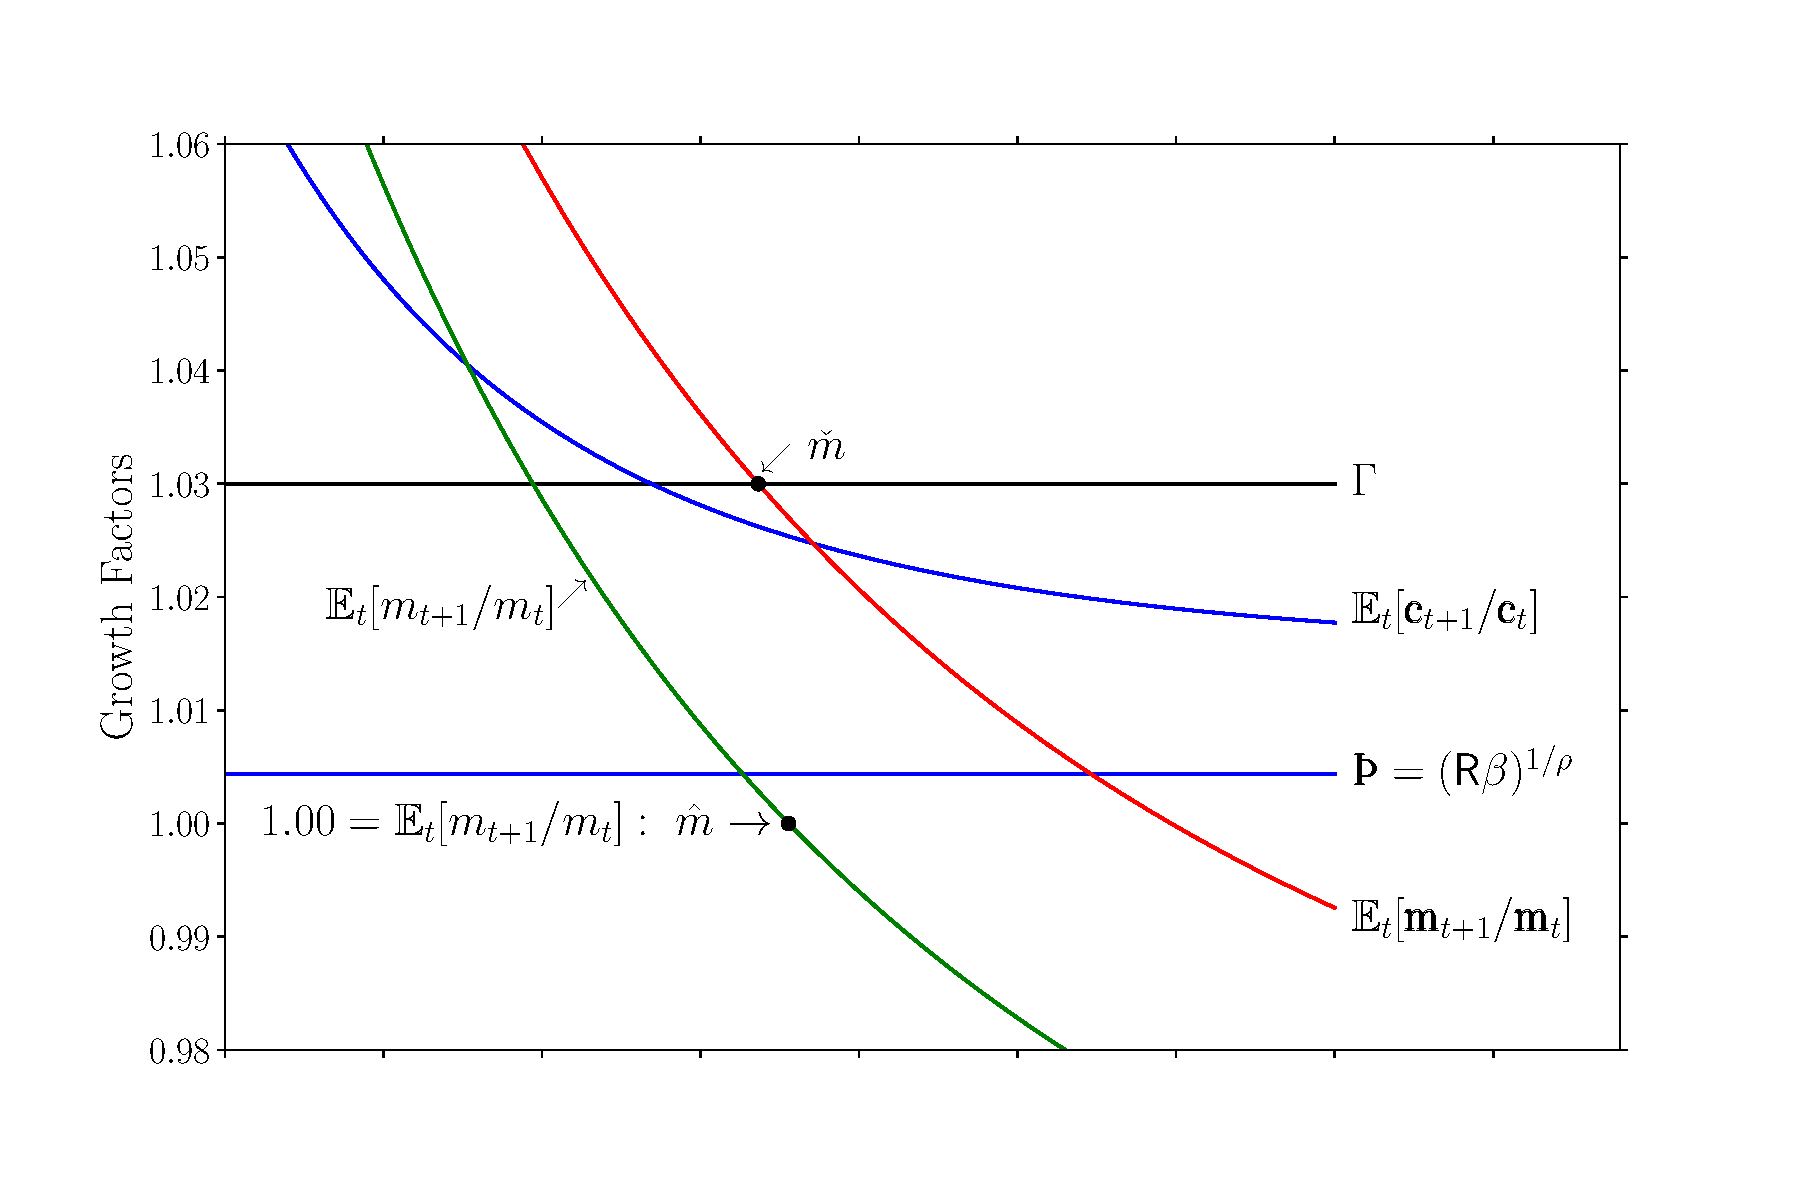
\includegraphics[width=4in]{\FigDir/cGroTargetFig.pdf}}
\end{frame}

\subsection{Bounds On The Consumption Function}
\begin{frame}
\frametitle{Bounds On the Consumption Function}
\centerline{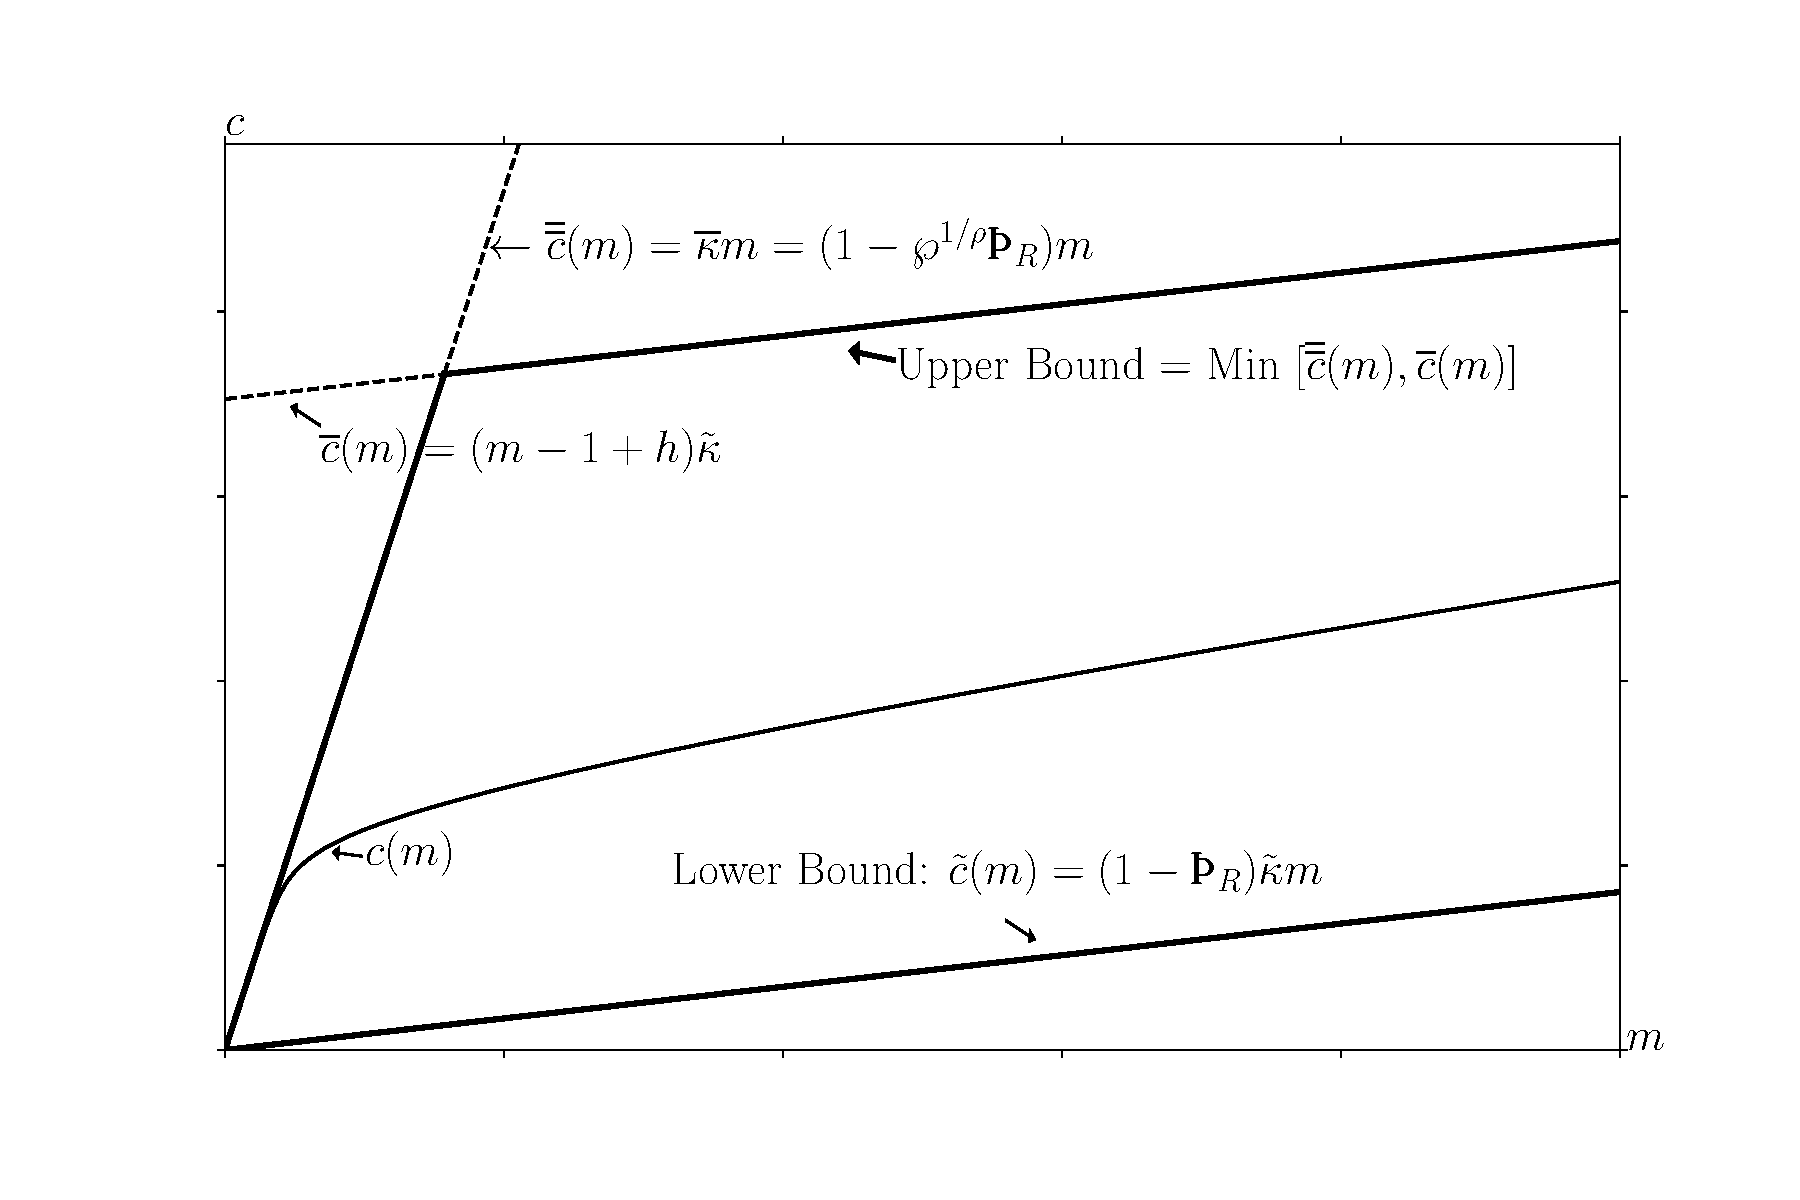
\includegraphics[width=4in]{\FigDir/cFuncBounds.pdf}}
\end{frame}

\begin{frame}
\frametitle{The Marginal Propensity to Consume}
\centerline{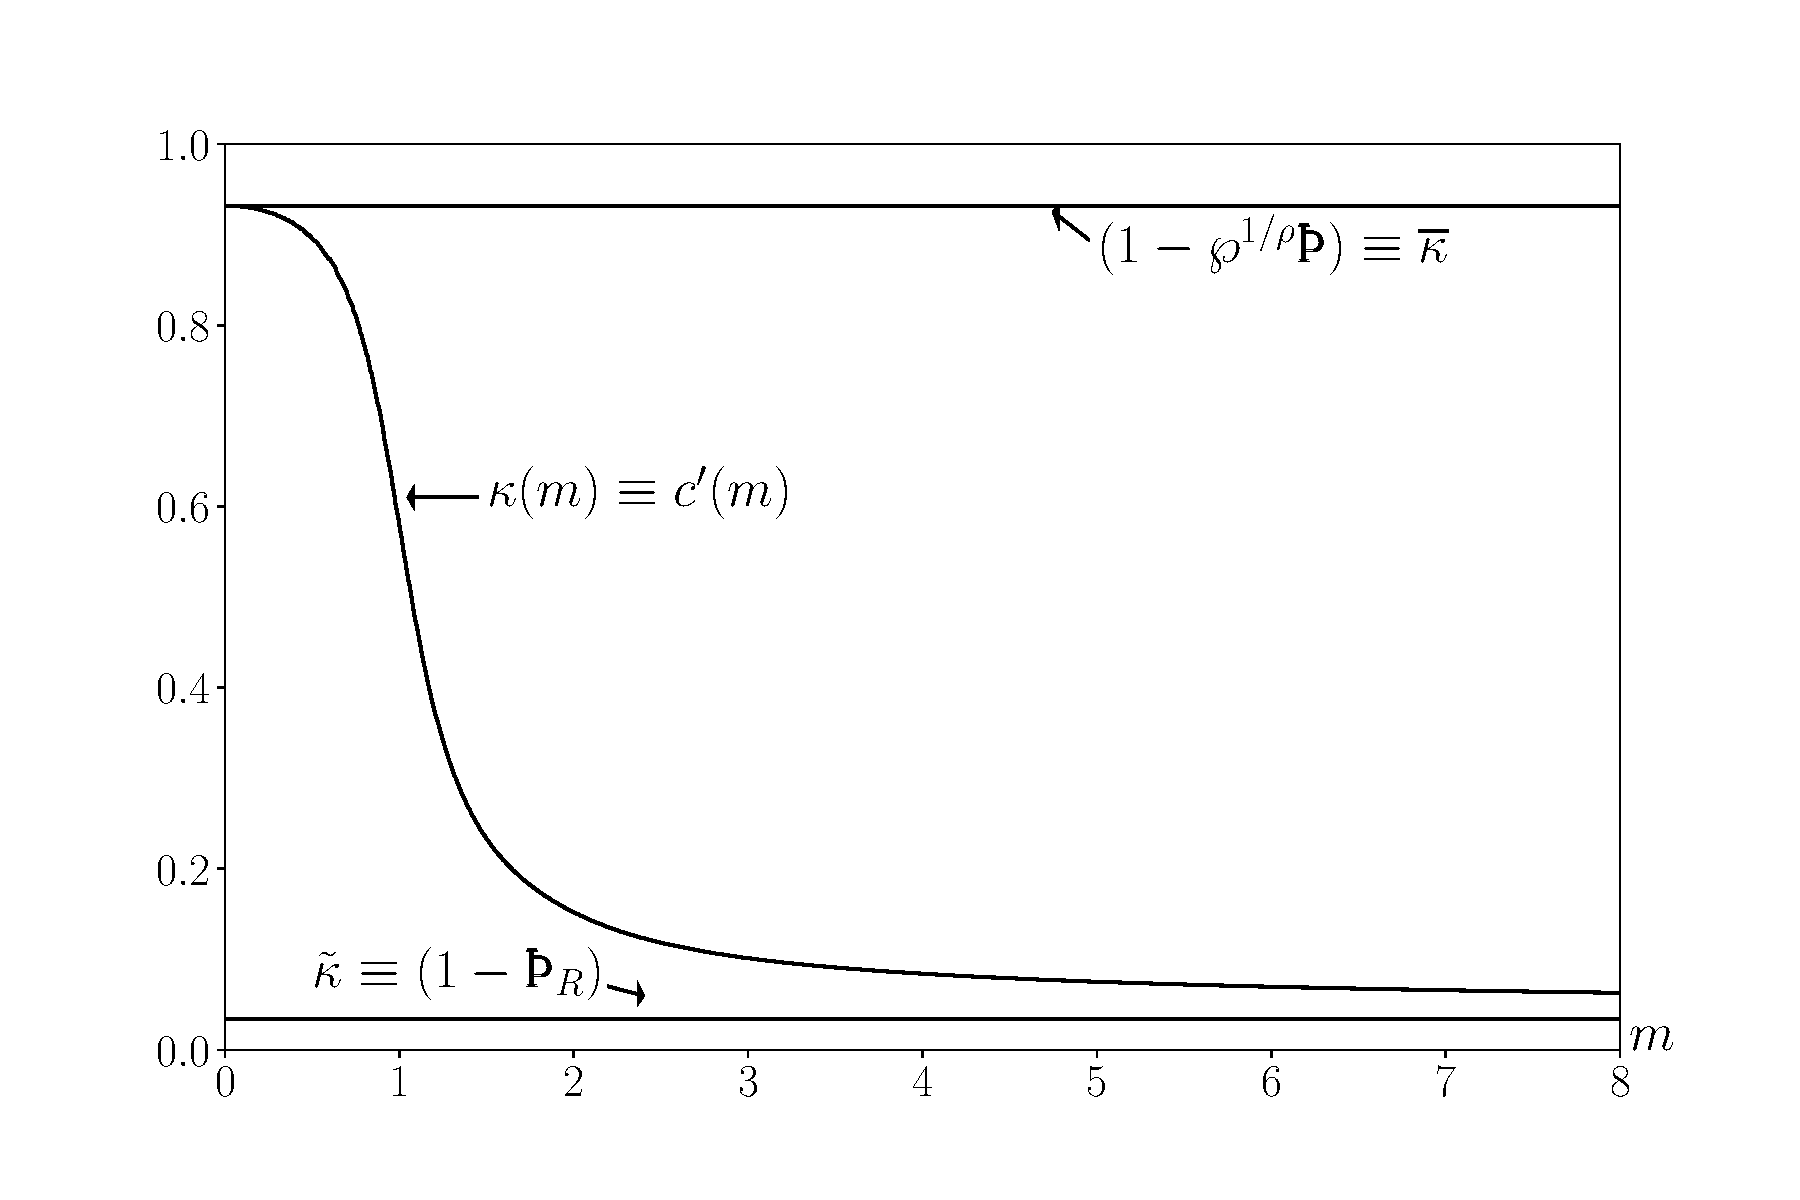
\includegraphics[width=4in]{\FigDir/MPCLimits.pdf}}
\end{frame}

\subsection{The Consumption Function and Target Wealth}
\begin{frame}
\frametitle{The Consumption Function and Target Wealth}
\centerline{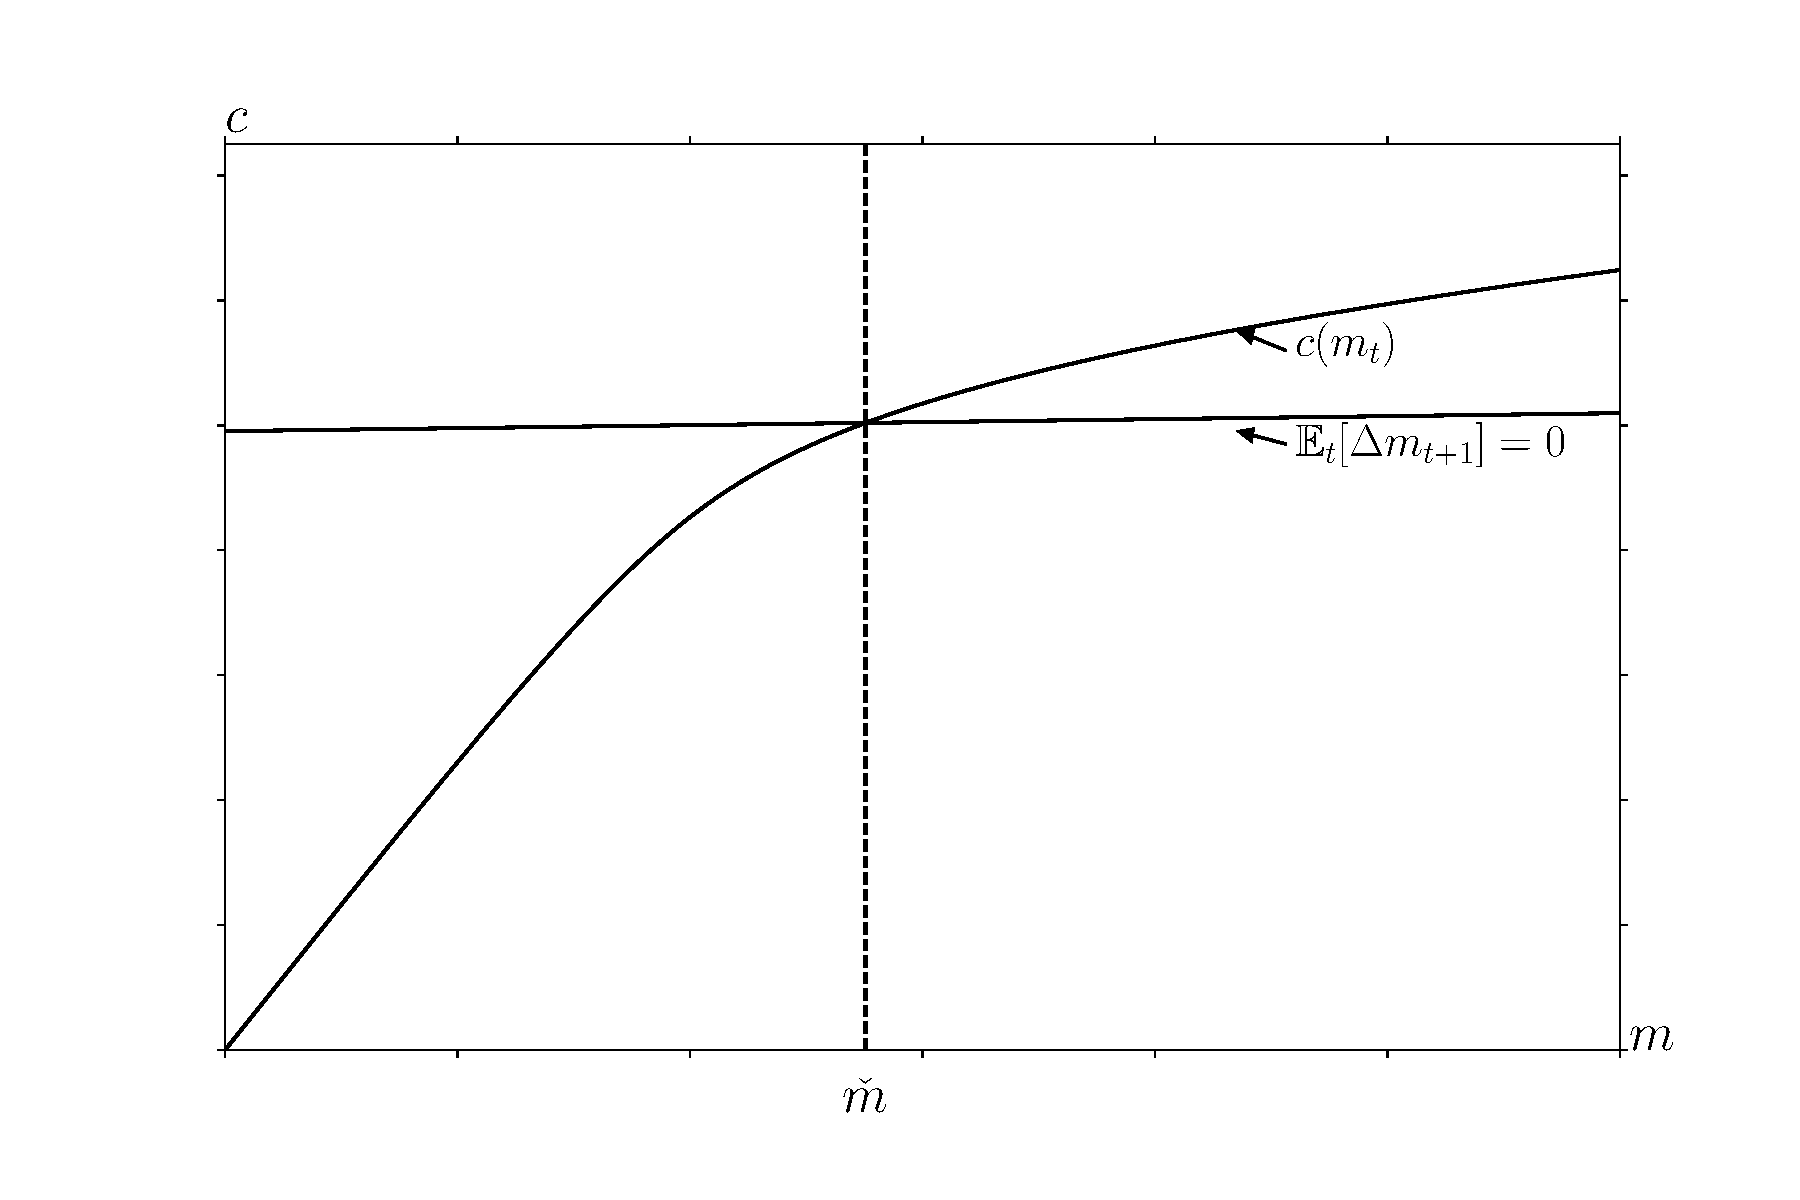
\includegraphics[width=4in]{\FigDir/cRatTargetFig.pdf}}
\end{frame}



\section{A Small Open Buffer Stock Economy}

\subsection{The Invariant Distribution}
\begin{frame}
\frametitle{Convergence To The Invariant Distribution}

\cite{szeidlInvariant} Proves Existence of an Invariant Distribution of 
$\mRat, \cRat, \aRat,$ etc.

\centerline{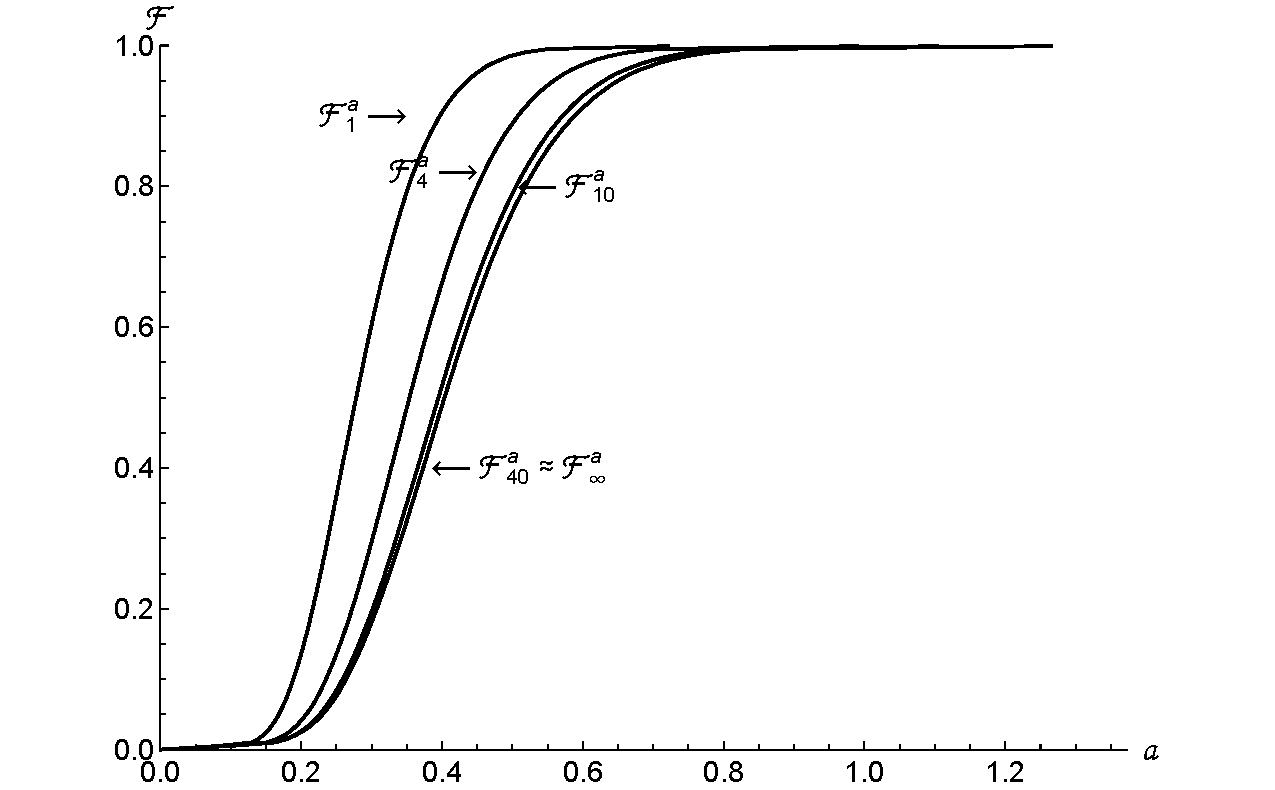
\includegraphics[height=2.5in]{\FigDir/SimCDFsConverge.pdf}}



\end{frame}


\subsection{Balanced Growth Equilbrium}
\begin{frame}
\frametitle{Balanced Growth Equilibrium}

Achieved When Cross Section Distribution Reaches Invariance
\begin{eqnarray}
  \YLev_{t+1}/\YLev_{t} = \CLev_{t+1}/\CLev_{t} & = & \PGro
\end{eqnarray}

Fisherian Separation Fails, Even Without Liquidity Constraints!
\medskip\medskip

\pause Insight:
\begin{itemize}
\item  Precautionary Saving $\approx$ Liquidity Constraints
\item If $\constr{\cFunc}(m)$ is solution for constrained consumer, 
\end{itemize}
\pause
\begin{equation}
\lim_{ \wp \downarrow 0} \cFunc(m;\wp) = \constr{\cFunc}(m)
\end{equation}


\end{frame}

\begin{frame}
\frametitle{The MPC Out Of Permanent Shocks}

\url{https://www.econ2.jhu.edu/people/ccarroll/papers/MPCPerm.pdf}
\medskip

Lots of Recent Papers Trying to Measure the MPCP

\medskip
Paper Proves:

\begin{itemize}
\item MPCP $< 1$
\item But not a lot less:
\begin{itemize}
\item 0.75 to 0.95 (annual rate) for wide range of parameter values
\end{itemize}
\end{itemize}

\end{frame}

\section{Conclusions}
\begin{frame}

\begin{itemize}
\item Defined Conditions Under Which Widely Used Problem Has Solution
\begin{itemize}
\item Finite Value of Autarky Condition Guarantees Contraction (with \WRIC)
\item Growth Impatience Condition Prevents $m \rightarrow \infty$
\end{itemize}
\item Economy Of Buffer Stock Consumers Exhibits Balanced Growth
\begin{itemize}
\item Even In Absence of General Equilibrium Adj of Interest Rate
\end{itemize}
\end{itemize}

\end{frame}

\def\newblock{\hskip .11em plus .33em minus .07em}

\begin{frame}

\renewcommand{\bibsection}{\subsubsection*{\bibname }}

\tiny 

% \bibliography{\econtexBib,\LaTeXGenerated/\texname}
\bibliography{BufferStockTheory,./LaTeX/economics}

\end{frame}

\end{document} 
% Local Variables:
% eval: (setq TeX-command-list  (remove '("Biber" "biber %s" TeX-run-Biber nil  (plain-tex-mode latex-mode doctex-mode ams-tex-mode texinfo-mode)  :help "Run Biber") TeX-command-list))
% eval: (setq TeX-command-list  (remove '("BibTeX" "%(bibtex) %s" TeX-run-BibTeX nil t                                                                              :help "Run BibTeX") TeX-command-list))
% eval: (setq TeX-command-list  (remove '("BibTeX" "%(bibtex) %s" TeX-run-BibTeX nil (plain-tex-mode latex-mode doctex-mode ams-tex-mode texinfo-mode context-mode) :help "Run BibTeX") TeX-command-list))
% eval: (setq TeX-command-list  (remove '("BibTeX" "%(bibtex) ../LaTeX/%s" TeX-run-BibTeX nil t :help "Run BibTeX")   TeX-command-list))
% eval: (add-to-list 'TeX-command-list	'("BibTeX" "%(bibtex) LaTeX/%s" TeX-run-BibTeX nil t :help "Run BibTeX") t)
% eval: (cond ((string-equal system-type "darwin") (progn (setq TeX-view-program-list '(("Skim" "/Applications/Skim.app/Contents/SharedSupport/displayline -b %n LaTeX/%o %b"))))))
% TeX-PDF-mode: t
% TeX-file-line-error: t
% TeX-debug-warnings: t
% LaTeX-command-style: (("" "%(PDF)%(latex) %(file-line-error) %(extraopts) -output-directory=LaTeX %S%(PDFout)"))
% TeX-source-correlate-mode: t
% TeX-source-correlate-start-server: 0
% TeX-parse-self: t
% End:
